
\subsection*{task 2.1 [5 points] \\[1ex] the dihedral group $D_3$}

\textbf{NOTE:} If you decide to give this task a try, then really try to solve it yourself! Those who do not like to- or cannot think for themselves may of course just go to wikipedia and look up the solution \ldots but what would you gain from that? 

The following are the six symmetries (three rotations and three reflections) of a unilateral triangle:

\begin{center}
\begin{tabular}{cc}
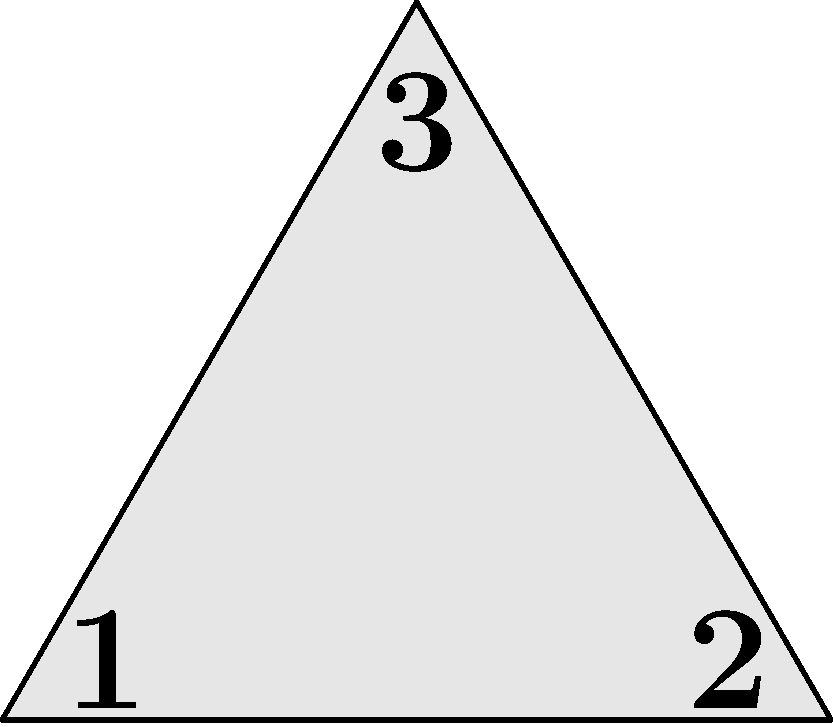
\includegraphics[width=0.1\textwidth]{triangle-I.pdf} \raisebox{2ex}{$\stackrel{I}{\rightarrow}$} 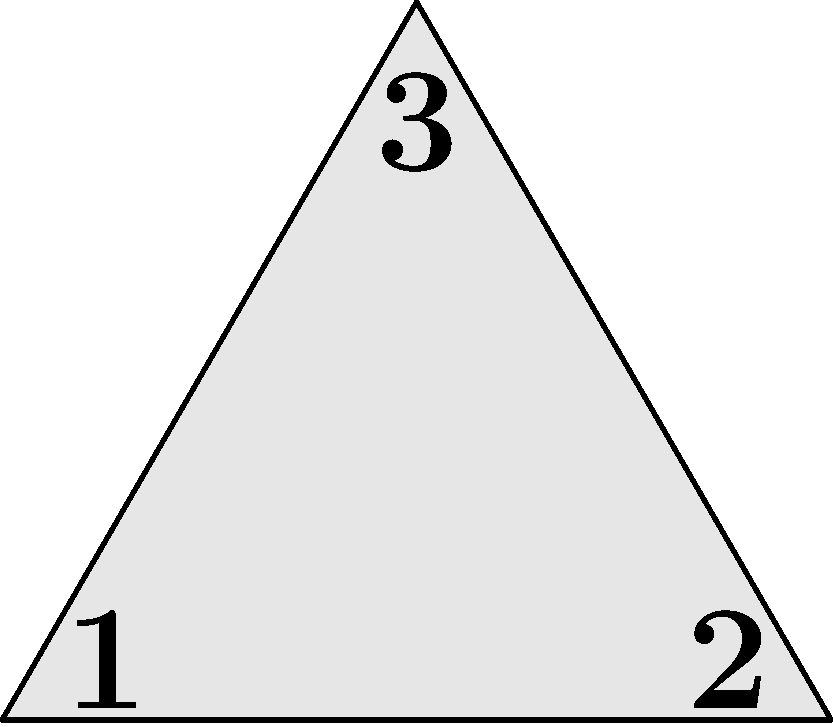
\includegraphics[width=0.1\textwidth]{triangle-I.pdf} \qquad
& \qquad 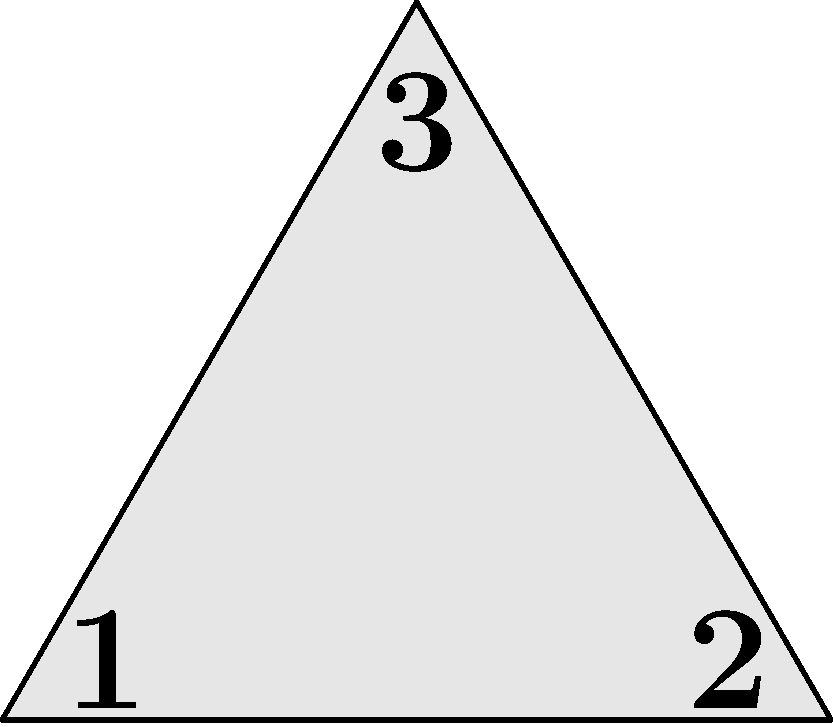
\includegraphics[width=0.1\textwidth]{triangle-I.pdf} \raisebox{2ex}{$\stackrel{F_1}{\rightarrow}$} 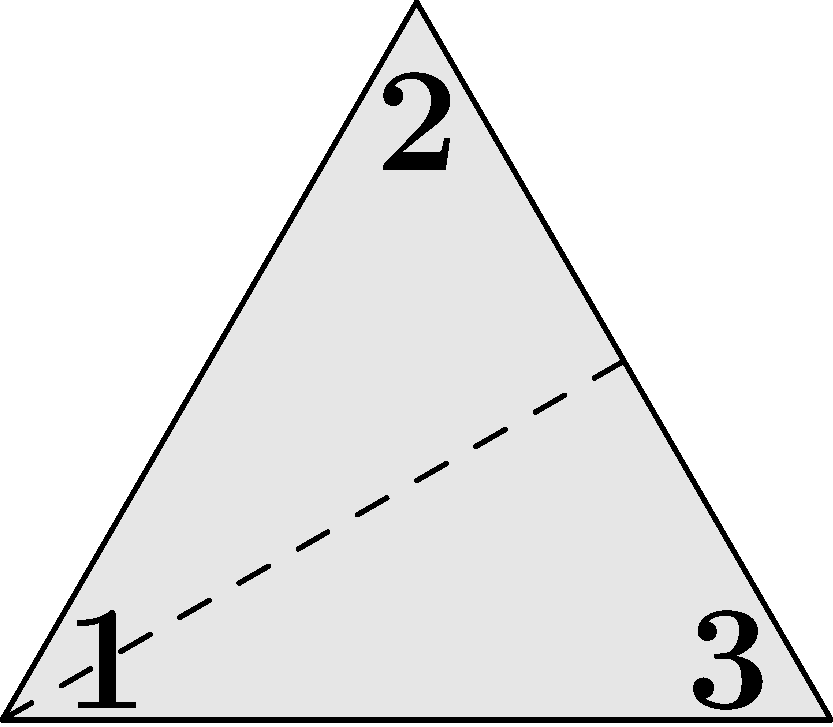
\includegraphics[width=0.1\textwidth]{triangle-F1.pdf} \\

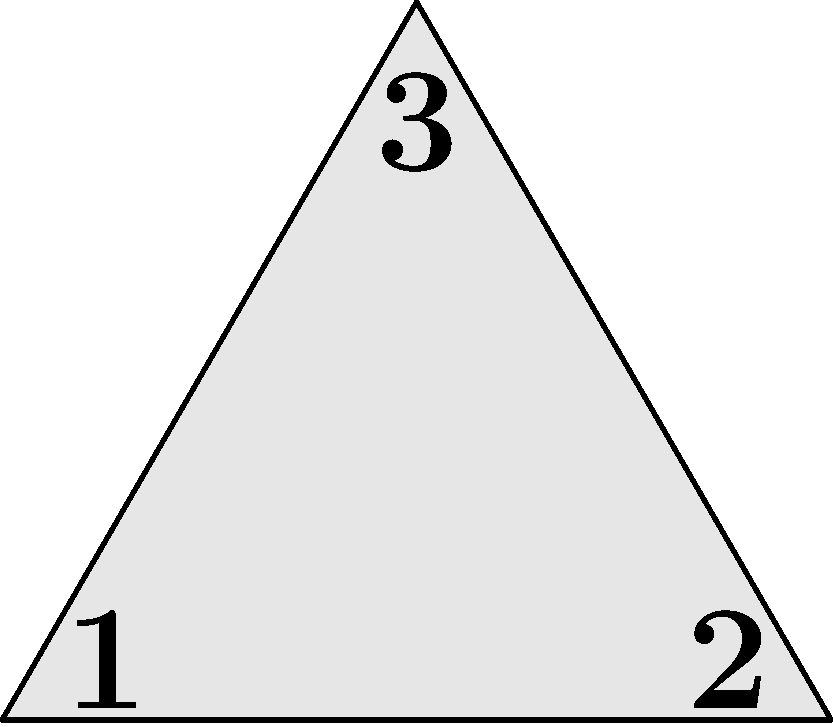
\includegraphics[width=0.1\textwidth]{triangle-I.pdf} \raisebox{2ex}{$\stackrel{R_1}{\rightarrow}$} 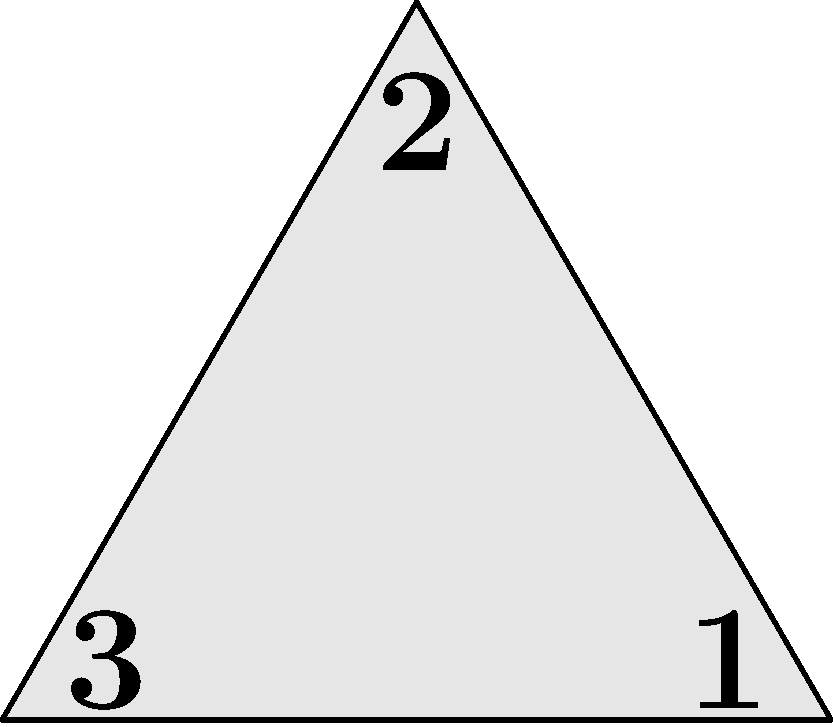
\includegraphics[width=0.1\textwidth]{triangle-R1.pdf} \qquad
& \qquad 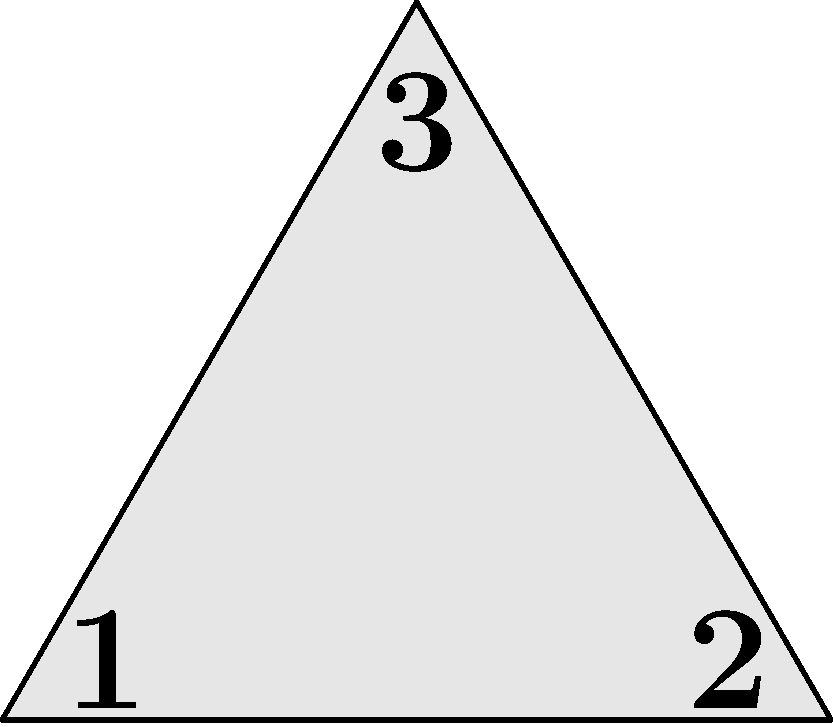
\includegraphics[width=0.1\textwidth]{triangle-I.pdf} \raisebox{2ex}{$\stackrel{F_2}{\rightarrow}$} 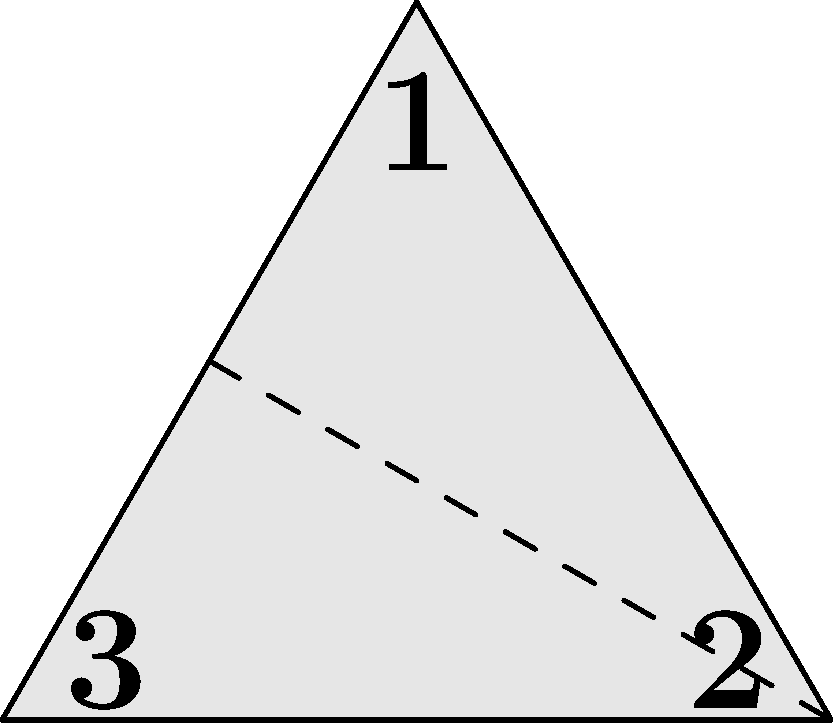
\includegraphics[width=0.1\textwidth]{triangle-F2.pdf} \\

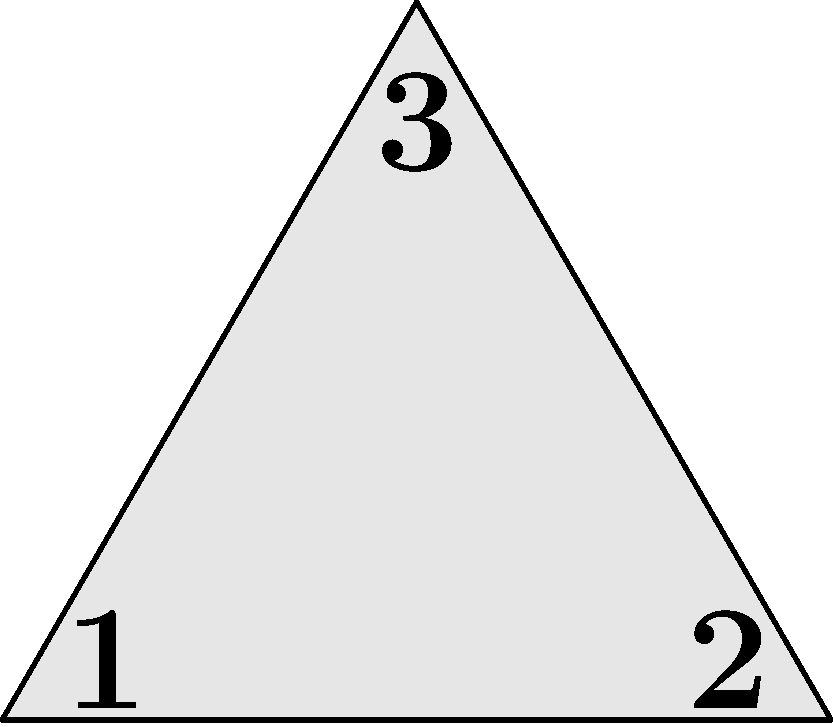
\includegraphics[width=0.1\textwidth]{triangle-I.pdf} \raisebox{2ex}{$\stackrel{R_2}{\rightarrow}$} 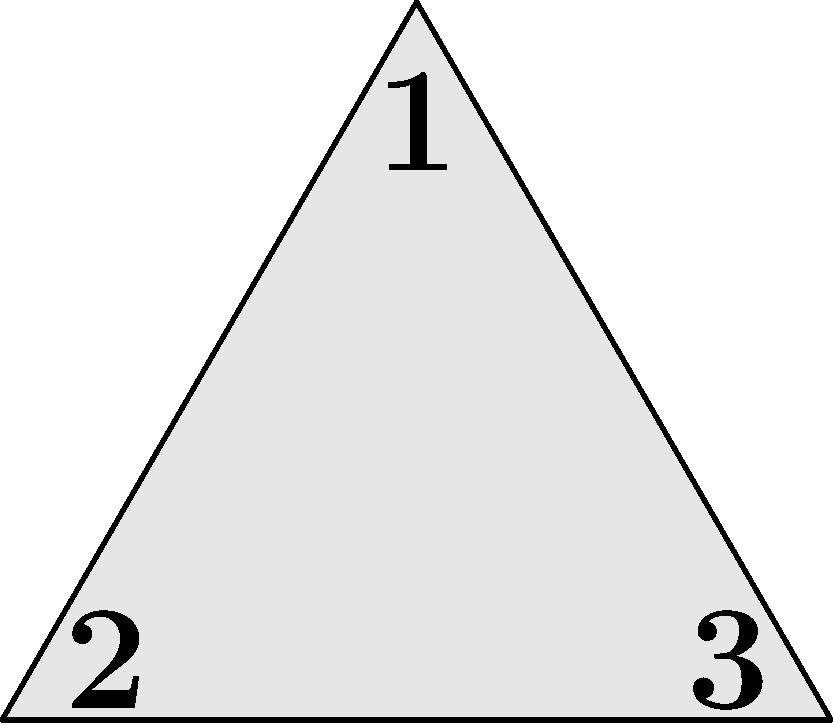
\includegraphics[width=0.1\textwidth]{triangle-R2.pdf} \qquad
& \qquad 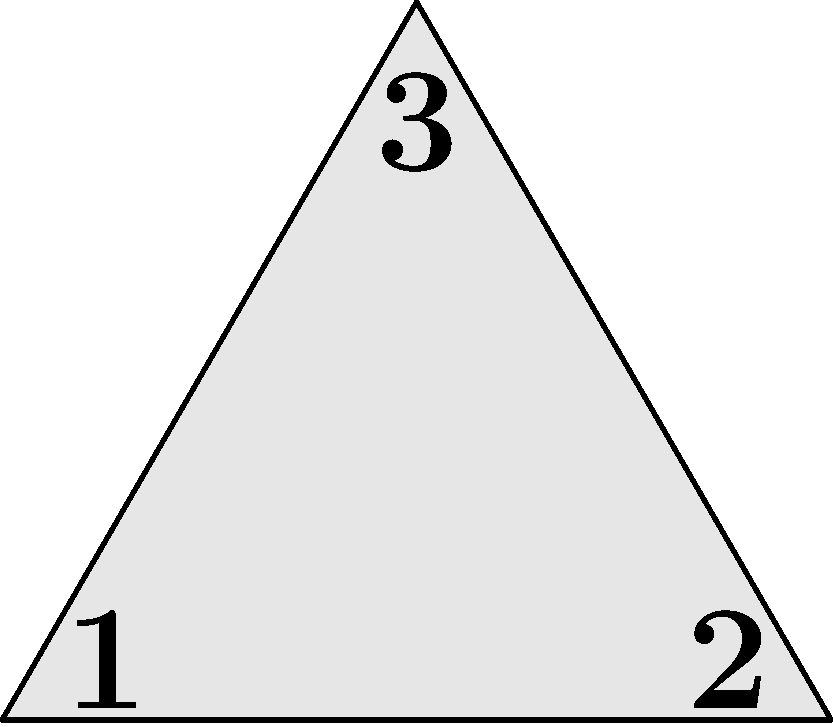
\includegraphics[width=0.1\textwidth]{triangle-I.pdf} \raisebox{2ex}{$\stackrel{F_3}{\rightarrow}$} 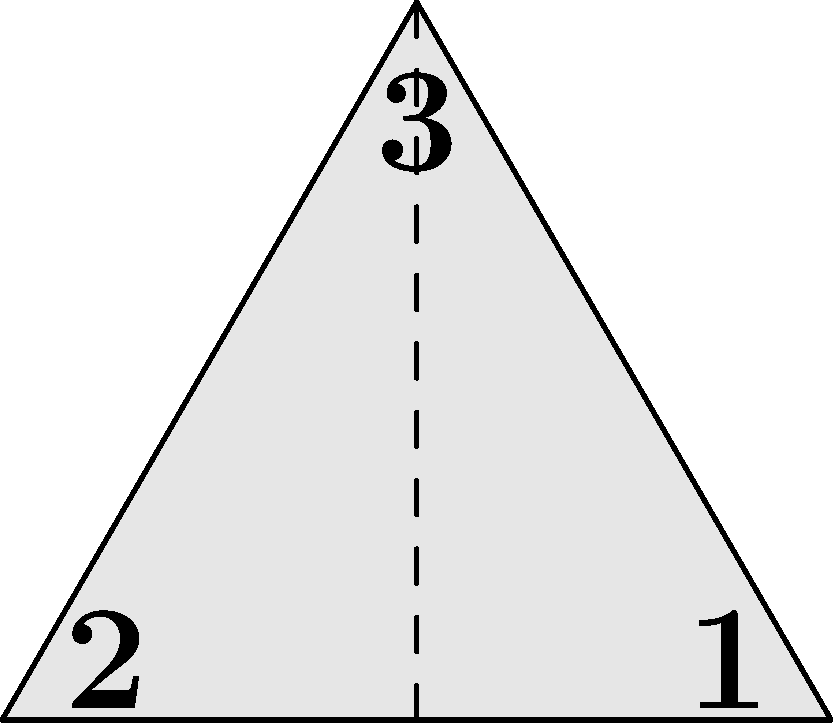
\includegraphics[width=0.1\textwidth]{triangle-F3.pdf}
\end{tabular}
\end{center}

Using the notation introduced in this figure, the dihedral group $D_3 = \bigl( G, \circ \bigr)$ consists of the following elements
\begin{align*}
G & = \bigl\{ I, R_1, R_2, F_1, F_2, F_3 \bigr\}
\intertext{and the group law}
\circ & \,:\, G \times G \rightarrow G
\end{align*}
is the composition, i.e. sequential execution, of any two operations in $G$. Given this information, complete the Cayley table for this group:
%%%%%
%%%%%
%%%%% complete the following table, i.e. replace the \ldots with the appropriate expression
%%%%%
%%%%%
\begin{center}
  \begin{tabular}{>{\columncolor[gray]{0.8}}cccccccc}
  \rowcolor[gray]{0.8} $\circ$ & $I$ & $R_1$ & $R_2$ & $F_1$ & $F_2$ & $F_3$ \\
  $I$   &  $I$  & $R_1$ & $R_2$ & $F_1$ & $F_2$ & $F_3$ \\
  $R_1$ & $R_1$ & $R_2$ &  $I$  & $F_2$ & $F_3$ & $F_1$ \\
  $R_2$ & $R_2$ &  $I$  & $R_1$ & $F_3$ & $F_1$ & $F_2$ \\
  $F_1$ & $F_1$ & $F_3$ & $F_2$ &  $I$  & $R_2$ & $R_1$ \\ 
  $F_2$ & $F_2$ & $F_1$ & $F_3$ & $R_1$ &  $I$  & $R_2$ \\
  $F_3$ & $F_3$ & $F_2$ & $F_1$ & $R_2$ & $R_1$ &  $I$   
  \end{tabular}
\end{center}
%%%%%
%%%%%
%%%%% complete the following table, i.e. replace the \ldots with the appropriate expression
%%%%%
%%%%%
\vspace{1ex}

Does your result ($\Leftrightarrow$ the structure of the completed table) suggest that $D_3$ is an Abelian group or not ?
\color{blue} \\[1ex]
%%%%%
%%%%%
%%%%% enter your discussion here
%%%%%
%%%%%
The Caylay table shows that the composition $\circ: G \times G \rightarrow G$ is not symmetric which implied that $D_3$ is not an Abelian group.
%%%%%
%%%%%
%%%%%
%%%%%
%%%%%
\color{black}
